\documentclass[11pt]{article}
\usepackage{apchem}
\doctitle{Unit 2 Content Guide}
\docsubtitle{A Comprehensive Review of Compound Structure and Properties, Topics 2.1--2.7}
\docstatus{Study draft}
\begin{document}
\titleblock
\begin{abstract}
This guide covers all of Unit 2, Compound Structure and Properties, in eight sections: one for each of Topics 2.1--2.7 in course order, plus a final section on lab skills and free-response technique. Each section gives the definitions, models and particle-level reasoning the topic needs, at least one worked example, the phrasing that earns free-response points and the mistakes that cost them. The worked examples use their own species, so none of them give away an item in \emph{Unit 2 Practice Set A} or \emph{Unit 2 Practice Set B}; the answer keys of both sets point back to the section numbers here. Plan on about 60 minutes for a full read. Draw every Lewis diagram in the worked examples yourself before reading the answer.
\end{abstract}
\leadline{Usage}{first pass, read Sections 1--8 in order and redo every worked example on paper. Then take \emph{Unit 2 Practice Set A} cold; reread the section behind every miss, and take \emph{Unit 2 Practice Set B} two or three days later. The last page is a one-page summary for the night before the unit test. Unit 2 is 7--9\% of the AP multiple-choice section, and Lewis diagrams and VSEPR appear in almost every free-response section.}

\section{Types of chemical bonds (Topic 2.1)}\label{t:2.1}
\subsection{Electronegativity decides the bond type}
\emph{Electronegativity} (EN) is an atom's pull on the electrons in a bond. It follows the trend in Unit 1: it rises across a period and falls down a group, with F the highest (4.0). The difference in EN between two bonded atoms places the bond on a continuum:
\begin{center}
\begin{tabular}{lll}\toprule
Bond type & Typical $\Delta$EN & Example \\ \midrule
Nonpolar covalent & about 0 (identical or near-identical atoms) & $\ce{Cl2}$, C--H (0.4) \\
Polar covalent & about 0.4 to 1.8 & O--H, C--Cl \\
Ionic & large, usually metal + nonmetal & NaF, $\ce{CaCl2}$ \\
Metallic & metal atoms only & Cu, Fe, brass \\ \bottomrule
\end{tabular}
\end{center}
\begin{itemize}
\item In a polar bond the more electronegative atom carries a partial negative charge ($\delta-$) and the other a partial positive charge ($\delta+$).
\item The boundary between polar covalent and ionic is not sharp. On the AP exam, ``metal + nonmetal'' is the working test for ionic bonding.
\item Compounds with polyatomic ions contain both kinds of bond: in $\ce{NH4Cl}$ the N--H bonds are covalent and the $\ce{NH4+}$--$\ce{Cl-}$ attraction is ionic.
\end{itemize}

\worked{1.1} Rank by polarity: C--F, C--Cl, C--Br. EN: F 4.0, Cl 3.2, Br 3.0, C 2.6. $\Delta$EN 1.4, 0.6, 0.4, so C--F $>$ C--Cl $>$ C--Br.

\worked{1.2} In an O--H bond, O is $\delta-$ and H is $\delta+$; in a B--H bond (B 2.0, H 2.2), the H is slightly $\delta-$. The more electronegative atom gets the negative end, whichever atom that is.

\errorsh
\begin{itemize}
\item Calling every bond between two nonmetals ``nonpolar.'' Check the EN difference.
\item Calling a compound with a polyatomic ion purely ionic.
\end{itemize}

\section{Intramolecular force and potential energy (Topic 2.2)}\label{t:2.2}
\subsection{The potential-energy curve of a bond}
As two atoms approach, the attraction of each nucleus for the other atom's electrons lowers the potential energy. If they get too close, nucleus--nucleus and electron--electron repulsion take over and the energy climbs steeply. The bond forms at the distance of lowest energy.

\begin{center}
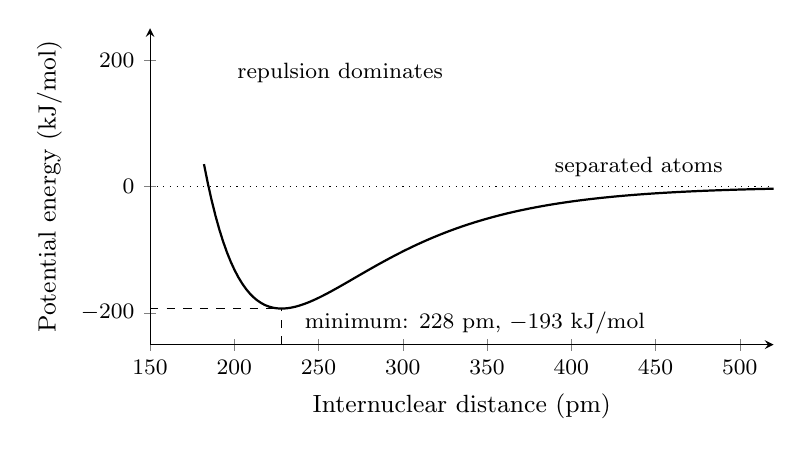
\begin{tikzpicture}
\begin{axis}[width=9.5cm,height=5.6cm,xmin=150,xmax=520,ymin=-250,ymax=250,axis lines=left,
  xlabel={Internuclear distance (pm)},ylabel={Potential energy (kJ/mol)},
  tick label style={font=\footnotesize},label style={font=\small},samples=150,domain=182:520]
\addplot[thick] {193*((1-exp(-0.016*(x-228)))^2-1)};
\draw[dashed] (axis cs:228,-250) -- (axis cs:228,-193);
\draw[dashed] (axis cs:150,-193) -- (axis cs:228,-193);
\draw[dotted] (axis cs:150,0) -- (axis cs:520,0);
\node[font=\footnotesize,anchor=west] at (axis cs:236,-215) {minimum: 228 pm, $-193$ kJ/mol};
\node[font=\footnotesize,anchor=west] at (axis cs:196,180) {repulsion dominates};
\node[font=\footnotesize,anchor=south] at (axis cs:440,0) {separated atoms};
\end{axis}
\end{tikzpicture}

{\small\itshape Potential energy of two bromine atoms. Bond length 228 pm; bond energy 193 kJ/mol.}
\end{center}
\begin{itemize}
\item \emph{Bond length}: the internuclear distance at the minimum.
\item \emph{Bond energy}: the depth of the well, the energy needed to separate the bonded atoms completely. Breaking a bond always requires energy; forming one releases it.
\item \emph{Atomic size}: larger atoms give longer bonds, usually with shallower wells (H--F 92 pm, H--I 161 pm).
\item \emph{Bond order}: more shared pairs give shorter, stronger bonds. C--C 154 pm, C=C 134 pm, C$\equiv$C 120 pm.
\end{itemize}

\worked{2.1} Two curves are drawn for $\ce{O2}$ and $\ce{N2}$. $\ce{N2}$ has a triple bond (order 3) and $\ce{O2}$ a double bond, so the $\ce{N2}$ minimum is at a shorter distance (110 vs.\ 121 pm) and is deeper (945 vs.\ 498 kJ/mol).

\worked{2.2} Coulomb's law also predicts the curve for an ion pair: $E \propto q_1q_2/r$. $\ce{Mg^2+}$ and $\ce{O^2-}$ at the same distance as $\ce{Na+}$ and $\ce{F-}$ have four times the attraction, because $(2)(2) = 4$.

\frph ``At the bond length the attractive and repulsive forces are balanced and the potential energy is at a minimum.'' To compare bond energies, compare well depths; to compare lengths, compare the positions of the minima, and give the reason (atom size or bond order).

\errorsh
\begin{itemize}
\item Saying a bond is broken ``to release energy.'' Bond breaking is always endothermic.
\item Thinking the zero of energy is the bonded state. Zero is the separated atoms.
\end{itemize}

\section{Structure of ionic solids (Topic 2.3)}\label{t:2.3}
An ionic solid is a three-dimensional lattice in which every ion is surrounded by ions of the opposite charge. There are no discrete molecules: the formula gives only the ratio of ions. The strength of the lattice comes from Coulombic attraction,
\[ F \propto \frac{q_+ q_-}{r^2}, \qquad r = r_+ + r_- , \]
so lattice strength (and melting point, hardness) increases with \emph{larger ion charges} and \emph{smaller ions}. Charge usually matters more than size.

\begin{center}
\begin{tabular}{lccc}\toprule
Compound & Ion charges & Ion sizes & Melting point (\textdegree C) \\ \midrule
KBr & $+1,-1$ & large & 734 \\
NaBr & $+1,-1$ & smaller cation & 747 \\
CaF$_2$ & $+2,-1$ & & 1418 \\
SrO & $+2,-2$ & & 2531 \\ \bottomrule
\end{tabular}
\end{center}
\textbf{Properties that follow from the model.}
\begin{itemize}
\item High melting points: many strong attractions must be overcome.
\item Brittle: shifting one layer lines up like charges, and repulsion splits the crystal.
\item Nonconducting as solids (ions fixed) but conducting when melted or dissolved (ions mobile).
\end{itemize}
\textbf{Particle diagrams.} Draw small cations and large anions in an alternating pattern; anions of halides are bigger than the matching cations in the same period. A diagram with like charges side by side, or with separate ``molecules,'' loses the point.

\worked{3.1} Rank by melting point: LiCl, LiF, BeO. BeO has $\pm2$ charges: highest. LiF vs.\ LiCl: same charges, $\ce{F-}$ smaller than $\ce{Cl-}$, so LiF is higher. Order: LiCl $<$ LiF $<$ BeO.

\errorsh
\begin{itemize}
\item Explaining with ``ionic bonds are stronger'' without naming charge and distance.
\item Saying ionic solids conduct because ``they have ions.'' The ions must be free to move.
\end{itemize}

\section{Structure of metals and alloys (Topic 2.4)}\label{t:2.4}
\subsection{Metallic bonding}
A metal is a lattice of cations in a ``sea'' of delocalized valence electrons. The bonding is nondirectional, which explains the properties:
\begin{itemize}
\item electrical and thermal conductivity: mobile electrons;
\item malleability and ductility: layers of cations slide without breaking the bonding;
\item luster: the delocalized electrons absorb and re-emit light.
\end{itemize}
More delocalized electrons per atom and smaller, more highly charged cores give stronger metallic bonding (Al $>$ Mg $>$ Na in melting point).

\subsection{Alloys}
\begin{center}
\begin{tabular}{p{0.19\linewidth}p{0.36\linewidth}p{0.36\linewidth}}\toprule
& Substitutional & Interstitial \\ \midrule
Atom sizes & similar radii & added atom much smaller \\
Where it goes & replaces host atoms in the lattice & fills holes between host atoms \\
Example & brass (Cu, Zn), sterling silver (Ag, Cu) & steel (Fe, C) \\
Effect & density changes; still malleable & harder, stronger, less malleable and ductile \\ \bottomrule
\end{tabular}
\end{center}

\worked{4.1} Atomic radii: Au 144 pm, Ag 144 pm, B 85 pm. Ag dissolves in Au as a substitutional alloy (equal sizes); B would enter the interstices.

\errorsh
\begin{itemize}
\item Saying metals conduct because ``the ions move.'' The cations stay put; the electrons move.
\item Mixing up the alloy types: interstitial means \emph{in the spaces}.
\end{itemize}

\section{Lewis diagrams (Topic 2.5)}\label{t:2.5}
\subsection{A reliable procedure}
\begin{enumerate}
\item Count valence electrons: add the group electrons of every atom, add one per negative charge, subtract one per positive charge.
\item Put the least electronegative atom in the center (never H; H forms one bond).
\item Connect the outer atoms with single bonds (2 electrons each).
\item Complete the octets of the outer atoms with lone pairs.
\item Put any remaining electrons on the central atom.
\item If the central atom has fewer than 8, turn outer lone pairs into double or triple bonds.
\end{enumerate}
\textbf{Exceptions.} H has 2 electrons; Be and B are often electron-deficient ($\ce{BeCl2}$, $\ce{BCl3}$); odd-electron species ($\ce{NO2}$, NO) cannot satisfy every octet; atoms in period 3 and below can expand their octets ($\ce{PF5}$, $\ce{SF4}$, $\ce{XeF2}$).

\worked{5.1} $\ce{NO2+}$: $5 + 2(6) - 1 = 16$ electrons. O--N--O uses 4; outer lone pairs use 12; N has only 4. Make two double bonds: O=N=O, with two lone pairs on each O.

\worked{5.2} $\ce{PCl3}$ vs.\ $\ce{PCl5}$: $\ce{PCl3}$ has 26 electrons, three bonds and one lone pair on P (octet). $\ce{PCl5}$ has 40, five bonds and no lone pair on P (10 electrons, an expanded octet).

\errorsh
\begin{itemize}
\item Forgetting to adjust for the charge of an ion, or adjusting in the wrong direction.
\item Leaving off lone pairs on outer atoms (``complete'' Lewis diagrams show all of them).
\item Expanding the octet of a period 2 atom: C, N, O and F never exceed 8.
\end{itemize}

\section{Resonance and formal charge (Topic 2.6)}\label{t:2.6}
\subsection{Resonance}
When a double bond or lone pair can be placed in more than one equivalent position, a single Lewis diagram cannot describe the species. The actual structure is a \emph{resonance hybrid}, an average of the resonance structures. It does not flip between them. Equivalent bonds in the hybrid are identical:
\[ \text{bond order} = \frac{\text{total bonding pairs between the central atom and the equivalent atoms}}{\text{number of equivalent links}}. \]
Nitrite, $\ce{NO2-}$, has two structures; each N--O bond has order 1.5. Benzene's C--C bonds all have order 1.5.

\subsection{Formal charge}
\[ \text{FC} = (\text{valence electrons}) - (\text{lone-pair electrons}) - \tfrac12(\text{bonding electrons}). \]
The formal charges in a structure add up to the charge of the species. When several structures are possible, the best one has
\begin{enumerate}
\item formal charges as close to zero as possible, and
\item any negative formal charge on the most electronegative atom.
\end{enumerate}

\worked{6.1} Cyanate, $\ce{OCN-}$ (16 electrons). Structure A: [O=C=N]$^-$, FC O 0, C 0, N $-1$. Structure B: [O--C$\equiv$N]$^-$, FC O $-1$, C 0, N 0. Structure C: [O$\equiv$C--N]$^-$, FC O $+1$, C 0, N $-2$. C is worst. B is best, because the $-1$ sits on O, the most electronegative atom; A also contributes.

\worked{6.2} The nitrite ion has bond order 1.5. Its N--O bonds (125 pm) are between an N--O single bond (about 140 pm) and an N=O double bond (about 120 pm).

\errorsh
\begin{itemize}
\item Describing resonance as the molecule ``switching'' between structures.
\item Counting all bonding electrons toward an atom's formal charge. Only half count.
\end{itemize}

\section{VSEPR and hybridization (Topic 2.7)}\label{t:2.7}
\subsection{Electron domains and shapes}
Each lone pair and each bond (single, double or triple) around the central atom is one \emph{electron domain}. Domains repel and spread as far apart as possible. The electron-domain geometry describes all domains; the \emph{molecular} geometry describes only the atoms.
\begin{center}
\small
\begin{tabular}{cllll}\toprule
Domains & Electron geometry & Lone pairs: molecular geometry & Angle & Hybrid. \\ \midrule
2 & linear & 0: linear & 180\textdegree & $sp$ \\
3 & trigonal planar & 0: trigonal planar; 1: bent & 120\textdegree, $<$120\textdegree & $sp^2$ \\
4 & tetrahedral & 0: tetrahedral; 1: trig.\ pyramidal; 2: bent & 109.5\textdegree, 107\textdegree, 104.5\textdegree & $sp^3$ \\
5 & trig.\ bipyramidal & 0: trig.\ bipyr.; 1: seesaw; 2: T-shaped; 3: linear & 90\textdegree, 120\textdegree & $sp^3d$ \\
6 & octahedral & 0: octahedral; 1: square pyramidal; 2: square planar & 90\textdegree & $sp^3d^2$ \\ \bottomrule
\end{tabular}
\end{center}
\begin{itemize}
\item Lone pairs repel more strongly than bonding pairs, so they shrink the bond angles ($\ce{CH4}$ 109.5\textdegree, $\ce{NH3}$ 107\textdegree, $\ce{H2O}$ 104.5\textdegree).
\item With five domains, lone pairs go in equatorial positions; with six, two lone pairs sit opposite each other.
\item The AP course stops at $sp^3$ for hybridization questions; $sp^3d$ and $sp^3d^2$ are listed only for completeness.
\end{itemize}
\subsection{Sigma and pi bonds}
A single bond is one $\sigma$ bond. A double bond is one $\sigma$ and one $\pi$; a triple bond is one $\sigma$ and two $\pi$. The $\pi$ bonds form from unhybridized $p$ orbitals, which is why an $sp^2$ atom can form one $\pi$ bond and an $sp$ atom two.
\subsection{Molecular polarity}
A molecule is polar if it has polar bonds \emph{and} a shape in which their dipoles do not cancel. Symmetric shapes with identical outer atoms ($\ce{CO2}$, $\ce{BF3}$, $\ce{CCl4}$, $\ce{PF5}$, $\ce{SF6}$, $\ce{XeF4}$) are nonpolar; lone pairs on the central atom or different outer atoms usually make a molecule polar.

\worked{7.1} $\ce{SF4}$: S has 6 valence electrons; four bonds use 4, leaving one lone pair: 5 domains, seesaw, polar.

\worked{7.2} Acetonitrile, $\ce{CH3CN}$. The $\ce{CH3}$ carbon has 4 domains ($sp^3$, 109.5\textdegree); the C$\equiv$N carbon has 2 ($sp$, 180\textdegree). Bonds: 3 C--H, 1 C--C and the C$\equiv$N give 5 $\sigma$ and 2 $\pi$.

\worked{7.3} $\ce{PCl3}$ is polar (trigonal pyramidal); $\ce{BCl3}$ is nonpolar (trigonal planar). The difference is the lone pair on P.

\frph Name the number of electron domains, the number of lone pairs, the shape, and then the consequence (angle, polarity). ``It is polar because it has polar bonds'' is not enough: the shape must keep the dipoles from canceling.

\errorsh
\begin{itemize}
\item Giving the electron geometry when the molecular geometry is asked for.
\item Counting a double bond as two domains.
\item Calling $\ce{CO2}$ polar because C=O is polar.
\end{itemize}

\section{Lab skills and free-response technique}\label{t:lab}
\subsection{Evidence for bonding type}
A lab may give you unknown solids and ask you to classify them. Use the properties together:
\begin{center}
\begin{tabular}{lcccc}\toprule
Test & Ionic & Metallic & Network covalent & Molecular \\ \midrule
Melting point & high & varies, often high & very high & low \\
Conducts as solid & no & yes & no (graphite yes) & no \\
Conducts melted / in water & yes & yes (melted) & no & no (unless it ionizes) \\
Hammered & shatters & flattens & shatters & crumbles \\ \bottomrule
\end{tabular}
\end{center}
\subsection{How this unit is tested in free response}
\begin{itemize}
\item ``Draw the complete Lewis electron-dot diagram'': every bond and every lone pair, with brackets and charge for ions.
\item Shape, angle and hybridization questions are usually one point each; give the name, not only a sketch.
\item Bond length and bond energy comparisons: cite bond order or atom size.
\item Melting-point comparisons for ionic solids: cite both ion charge and ion size (distance), and say which one decides.
\end{itemize}

\clearpage
\section*{Summary: Unit 2 on one page}
Use this page the night before. For any row you cannot explain from memory, reread its section and redo its worked example.

\begin{longtable}{@{}p{0.11\linewidth}p{0.40\linewidth}p{0.43\linewidth}@{}}\toprule
\S{} / Topic & Must know & Key ideas and tests \\ \midrule
1 / 2.1 & $\Delta$EN: nonpolar, polar, ionic; metallic; $\delta+$/$\delta-$ & metal + nonmetal = ionic \\[3pt]
2 / 2.2 & PE curve: length at minimum, energy = depth & higher order or smaller atoms: shorter, stronger \\[3pt]
3 / 2.3 & Lattice; brittle; conduct only when mobile & $F \propto q_+q_-/r^2$; charge first, then size \\[3pt]
4 / 2.4 & Electron sea; substitutional vs.\ interstitial & similar radii substitute; small atoms fill holes \\[3pt]
5 / 2.5 & Count electrons; octets; exceptions & period 2 never exceeds 8 \\[3pt]
6 / 2.6 & Resonance hybrid; bond order; formal charge & FC $= V - L - \tfrac12 B$; best: near 0, $-$ on most EN atom \\[3pt]
7 / 2.7 & Domains $\rightarrow$ shape; lone pairs shrink angles; $\sigma$/$\pi$; polarity & 2 $sp$, 3 $sp^2$, 4 $sp^3$ \\[3pt]
8 / lab & Properties identify the solid type & conductivity in solid and liquid \\ \bottomrule
\end{longtable}

\textbf{Shapes at a glance.}
\begin{center}
\begin{tabular}{lll}\toprule
Formula type & Shape & Example \\ \midrule
$\ce{AX2}$ & linear & $\ce{BeH2}$, $\ce{CS2}$ \\
$\ce{AX3}$, $\ce{AX2E}$ & trigonal planar, bent & $\ce{BCl3}$, $\ce{O3}$ \\
$\ce{AX4}$, $\ce{AX3E}$, $\ce{AX2E2}$ & tetrahedral, trigonal pyramidal, bent & $\ce{SiH4}$, $\ce{PH3}$, $\ce{H2S}$ \\
$\ce{AX5}$, $\ce{AX4E}$, $\ce{AX3E2}$, $\ce{AX2E3}$ & trig.\ bipyramidal, seesaw, T-shaped, linear & $\ce{AsF5}$, $\ce{SF4}$, $\ce{BrF3}$, $\ce{XeF2}$ \\
$\ce{AX6}$, $\ce{AX5E}$, $\ce{AX4E2}$ & octahedral, square pyramidal, square planar & $\ce{SeF6}$, $\ce{BrF5}$, $\ce{ICl4-}$ \\ \bottomrule
\end{tabular}
\end{center}
\end{document}
